\section{Google+}
\label{sec:google-plus}
Google+ znany również pod innymi nazwami takimi jak \emph{Google Plus} lub \emph{G+}, to serwis społecznościowy będący własnością firmy Google Inc.

Serwis ten podobnie jak Facebook, umożliwia dzielenie się informacjami między użytkownikami sieci poprzez możliwość zamieszczania tekstów, zdjęć, wideoklipów czy linków do innych zasobów w sieci, promując je własną marką lub nazwiskiem.

W sieci krąży bardzo wiele różnych wersji logotypu Google+ czy g+, które są często zmieniane i komponowane specjalnie pod kolorystykę i układ skórek witryn internetowych, jednak aby sprecyzować rzeczywisty wygląd logotypów przedstawiono na rysunku \ref{fig:logo-google} dwa rodzaje logotypów występujące oficjalnie na stronie Google+ (\url{https://plus.google.com/}).

\begin{figure}[!h]
\centering
\begin{subfigure}{.5\textwidth}
  \centering
  
\includegraphics[width=.4\linewidth]{images/googleplus_color.png}
  \caption{Logo tekstowe}
  \label{fig:sub1}
\end{subfigure}%
\begin{subfigure}{.5\textwidth}
  \centering
  \scalebox{0.7}
  {
      
\includegraphics[width=.4\linewidth]{images/google-plus-logo.png}
  }  
  \caption{Logo graficzne}
  \label{fig:sub2}
\end{subfigure}
\captionsource{Rodzaje logotypów występujących na witrynie Google+}{\url{https://plus.google.com/}}
\label{fig:logo-google}
\end{figure}

Spośród wszystkich portali społecznościowych Google+ odróżnia się od konkurencji tym, że pragnie stawiać na wiarygodność informacji dostarczanej od użytkowników\footnote{W myśl założeń firmy Google, użytkownika portalu reprezentuje jakaś rzeczywista osoba lub organizacja, przez co uwiarygadnia dany podmiot. Osoby lub firmy nie będące fikcyjnym tworem przesyłając informacje, opinię, uwagę, ect. wnoszą pozytywny wkład w ogólny przekaz informacji, a nie sztuczną bańkę informacyjną ,,produkowaną i przekazywaną dalej'' w sieć, jako zabieg marketingowy do szybszego i skuteczniejszego wpływania na działania użytkowników.} oraz lokalność.

Umieszczenie informacji, zdjęć, nagrań wideo nie są jedynymi działaniami jakie oferuje g+. Portal pozwala także na tworzenie wydarzeń, opiniowanie produktów czy usług oferowanych przez firmy promujące się w społeczności poprzez rozdawanie plusików, a także integralny dostęp do innych usług oferowanych przez firmę Google zwiększając tym samym ofertę przystąpienia do społeczności.

%-----------------------------------------

\subsection{Promocja firmy, a Google+}
W chwili obecnej tj. 2 kwartale 2014 roku wyszukiwarka Google zajmuję 1 miejsce wśród narzędzi do wyszukiwania informacji w Polsce (95,59\% udziału rynku), zaraz za nią MSN (2,57\%) oraz Yahoo (0,97\%) \cite{url:gemius-ranking-silnikow-wyszukiwarek}.

Google będąc największym potentatem rozwiązań wyszukiwania informacji w internecie na polskim rynku można pokusić się nawet o stwierdzenie że jest niemal monopolistą rynkowym, spychając rywali na wąski margines.

Tak ogromny udział w rynku zapewnia niemal nieograniczone możliwości kreacji promocji w sieci. Jednak z punktu widzenia wolności i konkurencyjności rynku, ,,wyszukiwarek'' baron dyktuje koszty promocji wszystkim tym, którzy korzystają z jego produktów --- a jest to niemal całość polskiego społeczeństwa $\sim$96\%. Tak wielki procent udziałów w rynku, poniekąd zmusza firmy do skorzystania z oferty Google, jeśli chcą dotrzeć do większości polskich internatów. \\


Jednym z darmowych narzędzi ułatwiających promocję firmy wśród mediów społecznościowych jest wcześniej wspomniany google+. Google+ jako jedna z usług dostarczanych przez firmę Google ma za zadanie łączyć społeczność portalu i personalizować ich użytkowników, a przez to uwiarygadniać oraz dzielić się treściami pochodzącymi z wiarygodnego, zaufanego źródła --- przykładowo naszego przyjaciela Pana Michała, który istnieje (nie jest fikcyjną wykreowaną przez media/marketing postacią) i wyraził swoją opinię o jednym z przedmiotów promowanych przez firmę. Dzięki sieci Google+ wiem z dużym prawdopodobieństwem, że opinia Pana Michała jest wiarygodna, ponieważ go znam (widuję na co dzień), a dzięki dobrej opinii o wykonaniu usługi istnieje również większa szansa, że i ja skorzystam z usługi.\\

Ta krótka, lecz ważna notka z punktu widzenia osoby prawnej, w wąskim stopniu przybliża działanie idei portalu oraz istotności potrzeby promocji w nim (a także wszystkich usługach oferowanych przez Google, które poniekąd tworzą jedną spójną całość uzupełniając się wzajemnie). 

Rozmawiając o usłudze Google+ dyskutujemy tak na prawdę o narzędziu spajającym ze sobą pozostałe usługi dostarczane przez firmę Google w postaci jednego, ułatwiającego zarządzanie Panelu Google+.

%-------------------------------------------

\subsection{Panel Google+}
Panel Google+ to obszar skupiający w jednym miejscu kluczowe informacje dotyczące różnych obszarów istotnych w prowadzeniu firmy w internecie (tu celowo pomijam użytkownika indywidualnego, ponieważ nie jest on tematem dysputy w niniejszej publikacji).\\

\begin{figure}[!h]
\centering
    \scalebox{0.21}
    {
        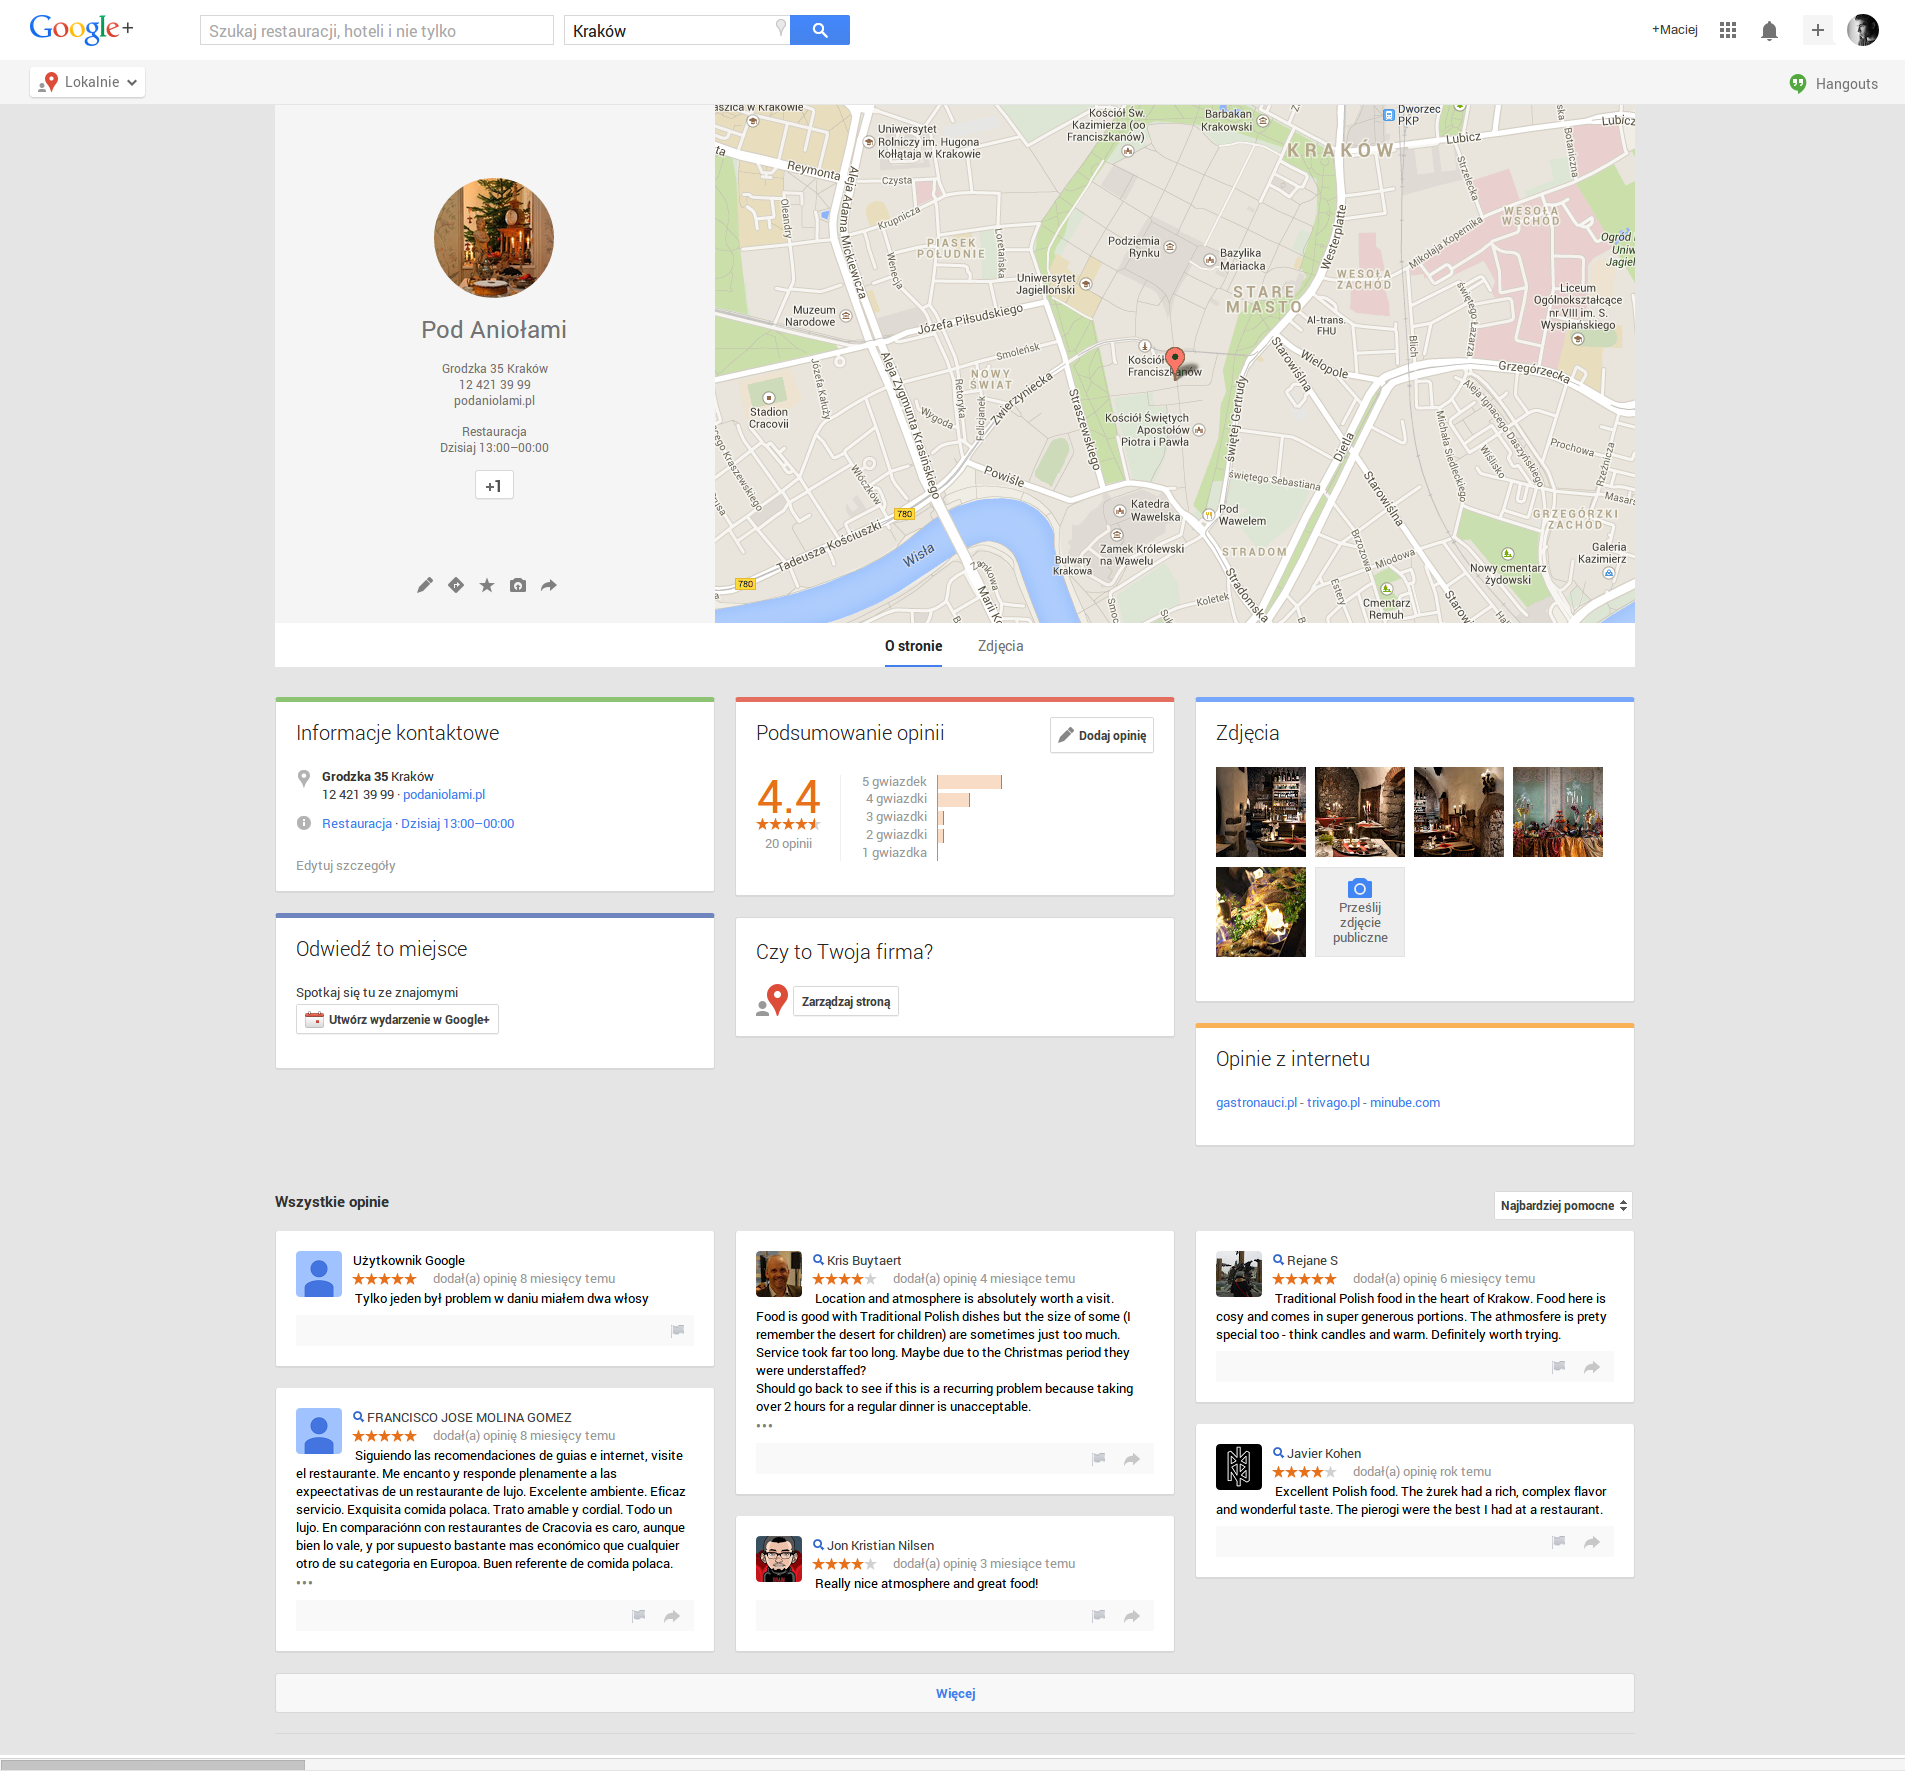
\includegraphics{images/pod-aniolami-google-plus.png}
    }
    \captionsource{Przykładowy profil firmy w Google+}{Opracowanie własne}
    \label{fig:sample-google-plus-company-profile-page}
\end{figure}

Panel Google+ dostarcza m.in:

\begin{itemize}
\item Możliwość aktualizacji danych firmy w 1 miejscu;

\item Narzędzia sprawdzające kompletność i zgodność witryny z wyszukiwarką \mbox{Google};

\item Wyświetlać wpisy innych użytkowników oraz tworzyć własne z informacjami, zdjęciami i filmami.

\item Szeroka interakcja z klientami poprzez budowanie precyzyjnego grona odbiorców oraz udoskonalanie swoich zasobów odpowiadając na opinie użytkowników o firmie/usłudze.

\item Rozmawiać bezpośrednio ,,twarzą w twarz'' z klientami dzięki usłudze Google Hangouts (internetowy odpowiednik Skype lub Viber);

\item Przeglądać szeroki zakres różnego typu statystyk dotyczących firmy a w tym:
    \begin{itemize}
    \item Najpopularniejsze wyszukiwania na temat firmy w wyszukiwarce Google;
    \item Skąd klienci wyznaczą trasy dojazdu do placówki dzięki usłudze Google Maps;
    \item Sprawdzenie popularności firmy wśród społeczności Google+;
    \end{itemize}

\item Zarządzać reklamami, w tym także poprzez integrację z usługą AdWords Express;

\item Mobilność dostarczanych rozwiązań (Smartphone, Tablet, Komputer);
\end{itemize}

%----------------------------------------------------------------------

\subsection{Możliwości promocji w Google+}
Model promocji działalności w Google+ jest dość jasny --- tworząc własny profil lub inaczej stronę (ang. \textit{wall}) umieszczamy wszystkie rzeczy dotyczące firmy tj. informacje oraz mapę dojazdu do firmy, tworzymy posty z atrakcyjnymi ofertami usługami lub produktów, a w zamian uzyskujemy ogromne i w miarę możliwości wiarygodne\footnote{Wiarygodność jest tu ujęta w cudzysłów, ze względu na fakt, iż prawdopodobnie nigdy nie osiągnie poziomu 100\%. Zawsze jakiś odsetek opinii czy uwag na temat produktu będzie przejaskrawiony w negatywną stronę lub po prostu zrobiony z premedytacją (w ramach zagrań nieczystej konkurencji).\\ Jednak ogólne założenia wiarygodności użytkowników w systemie Google+ pozwalają nam z dużym prawdopodobieństwem twierdzić, że opinia danego klienta jest jak najbardziej prawdziwa i wartościowa, tak więc rozsądnie jest brać je wszystkie pod uwagę.} miejsce zwrotów opinii wśród użytkowników, który skorzystali z naszych usług. 

\noindent Dodatkowo dzięki informacji zwrotnej od klientów (posiadających konto Google+) możemy szybko skorygować lub udoskonalić naszą ofertę, a tym samym promując ją dalej wśród znajomych naszych klientów, którzy właśnie skorzystali z części naszej oferty i wyrazili opinię. 

Jak widać na rysunku \ref{fig:sample-google-plus-company-profile-page} przedstawiającym schludny, stonowany, firmowy profil Google+ jednej z Krakowskich restauracji, który posłuży nam jedynie jako wstępny szablon informacji o modelach promowania się wraz z siecią google+.

To jednak tylko ogólny zarys wstępu do poszczególnych kanałów jakie oferuje Google+. W dalszej części omówimy bardziej szczegółowo poszczególne możliwości usługi w nieco szerszym zakresie, w tym profity jakie niosą ze sobą dla inwestora chcącego dowiedzieć się co uzyska (lub straci) dzięki takiemu profilowi.


%-------------------------------------------

\subsubsection{Jak wykorzystać strony Google+ w biznesie?}
Istnieje wiele różnych sposobów do wykorzystania stworzonego profilu w systemie Google+, wśród których można wyróżnić kilka skupiających się w około \cite[s.119]{Brogan12}:

\begin{itemize}
\item Narzędzia edukacyjnego;
\item Kanału użytkowników;
\item Platformie komunikacyjnej;
\item Centrum medialnemu;
\item Przestrzeni współpracy i wymiany danych;
\end{itemize}

Każdy z powyższych przykładów rządzi się swoimi prawami, zaletami i wadami płynącymi z prowadzenia określonej struktury profilu. Trudno tu faworyzować konkretne rozwiązanie, ponieważ wybór charakteru wykorzystania profilu winien być świadomy i równoważny, równoważący bądź uzupełniający wykorzystanie innych kanałów mediów społecznościowych, gdyż każde medium jest swoistą odmianą komunikacji panującej między użytkownikami\footnote{Jeden  z portali społecznościowych służy jako wymianie wiedzy, drugi jako informator dla lokalnej społeczności, a trzeci może wyłącznie skupiać się na relacjach biznesowych}.

O tym jakie drogi mogą umożliwić promocja w medium społecznościowym \mbox{Google+} zostanie przybliżona w kolejnych sekcjach. Przeanalizujemy przykładowe modele i możliwości płynące z ich wykorzystania w różnych sytuacjach.

%-------------------------------------------

\subsubsection{\nmu Wszystko w jednym miejscu}
\label{subsubsec:wszystko-w-jednym-miejscu}
Dla wielu rekinów biznesu ale i nie tylko, pewne przysłowie: ,,jak coś jest  do wszystkiego, to jest do niczego'' jest jak najbardziej prawdziwe i sprawdza się. Jednak w tym kontekście naszego podrozdziału \lnameref{subsubsec:wszystko-w-jednym-miejscu}, główna strona profilu\footnote{Nota bene profil Google+ inaczej widzi właściciel konta, ponieważ posiada możliwość edycji materiałów na profilu, a nieco odmiennie widzi go klient lub po prostu inny użytkownik portalu google+, który może zaobserwować zwartą kondensacje danych w postaci prostej przewijanej witryny (aktualnie popularny i obserwowalny w internecie model tworzenia witryn www nie wymagający za dużo ,,męczenia się i klikania'', a jedynie oczekuje od użytkownika przewijanie strony coraz niżej --- taki rozwój stron może być nawet traktowany jako kompensacja rozwoju internetu)}, czyli tak zwany \textit{wall} zawiera wszystkie najpotrzebniejsze informacje dla klienta co widać na rysunku \ref{fig:sample-google-plus-company-profile-page} i w tym kontekście powinna być rozpatrywana. Nie jako narzędzie do wszystkiego, chodź za takie może uchodzić ponieważ jest elementem łączącym pozostałe usługi firmy Google przykładowo tj. Hangouts, Google Maps czy AdWords. 

\noindent Jednak oprócz spoiwa różnych usług, którym z pewnością jest google+, zapewnia również interakcję z użytkownikiem poprzez umieszczanie postów (w tym tekstu, obrazu, wideo) oraz wydawanie opinii klientów o swoich usługach. 

W głównej mierze ma być miejscem profesjonalnej i rzetelnej informacji dla klienta. Pytanie tylko czy stosunkowo niedawne wejście na rynek pozwoli poważnemu i profesjonalnemu Google+ wyprzeć bardziej frywolnego, kierowanego na luźniejsze relację giganta jakim jest Facebook\footnote{Firma Google posiada nieco odmienne założenia społecznościowe dla swoich produktów. Google stawia na wiarygodności i rzetelność opinii na których można polegać i równie dobrze szybko odnaleźć (dzięki lepszej współpracy z własną wyszukiwarką). To są niepodważalne cechy profesjonalizmu dla firm. 
Flagowy produkt firmy Facebook skupia się natomiast na nieco innych założeniach. Mianowicie relacjach międzyludzkich głęboko zakorzenionych w ludziach jak np.: związkach(słynny status ,,w związku''), przyjaźniach, dzieleniem się informacjami w bliskim kontakcie z przyjaciółmi. Model produktu Facebook moim zdaniem ma zastosowanie dla nieco odmiennej grupy firm, niż bardziej uniwersalny Google+, co nie oznacza że zamyka im drogę. Jednak nie wszystko co związane z firmą, w oficjalny sposób można wrzucić na Facebook z racji różnego modelu świadczonych usług obydwu produktów.}.

%--------------------------

\subsubsection{Budowanie społeczności}
Wielokrotnie wspominany profil w Google+ w dostarcza wielu różnych usług pomagających w relacjach społecznościowych.

\begin{figure}[!h]
\centering
    \scalebox{0.25}
    {
        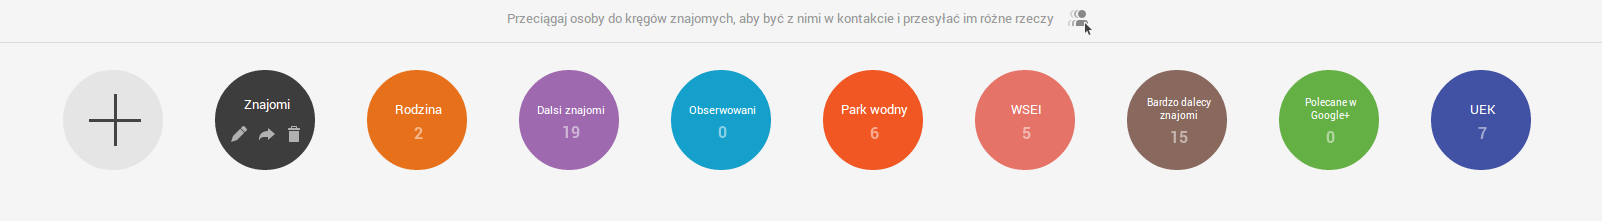
\includegraphics{images/google-plus-circles.png}
    }
    \captionsource{Kręgi w Google+}{Opracowanie własne}
    \label{fig:google-plus-circles}
\end{figure}

Jedną z nich są Kręgi (ang. Circles) i przykładowy zrzut ekranu z widokiem znajdziemy na rysunku~\ref{fig:google-plus-circles}. To usługa pozwalająca budować grupy kontaktów i tym samym tworzyć łatwe połączenia (w szczególności biznesowe) zanim będziemy próbować sprzedać swój produkt dalej. To ważne dla wielu osób (z punktu widzenia psychologicznego również) z tego względu, że tworzy ,,wrażenie znajomości'' mimo iż np.: w rzeczywistości nie miała ona miejsca.
Wtedy łatwiej o nawiązanie kontaktu, a jeśli ktoś ma go z swoich kontaktach i spodoba się to efekt domina rozprzestrzenia się samoistnie --- to bardzo prosta i przydatna rzecz podczas promocji własnej firmy dalej w świat.

Jest kilka strategi budowania społeczności Google+, lecz nie będą one głównym tematem tej dyskusji. To co jest istotne dla właściciela przyszłego konta Google+ Business to rozróżnienie 2 grup, które występują w kontaktach i można je zaobserwować na rysunku \ref{fig:size-of-audience-in-google-plus-circles}. 

\begin{figure}[!h]
\centering
    \scalebox{0.7}
    {
        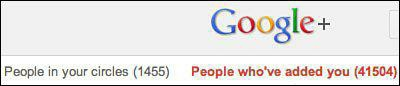
\includegraphics{images/size-of-audience-in-google-plus-circles.png}
    }
    \captionsource{Ilość osób w kręgach}{\cite[s.96]{Brogan12}}
    \label{fig:size-of-audience-in-google-plus-circles}
\end{figure}

Pierwszą z nich jest \emph{liczba osób w Twoich kręgach} oraz \emph{osoby, które dodały Cię do swoich kręgów}. Jak na razie sprawa jest bardzo prosta i intuicyjna. Jednak Google w budowaniu sieci połączeń nałożył pewne restrykcje ograniczając liczbę osób we własnych kręgach do 5000 i jest to najważniejsza grupa z punktu widzenia prowadzenia profilu. Druga grupa (tj. osoby, które  dodały nasz profil do swoich kręgów) może mieć nieograniczone rozrastanie i można tą grupę określić w skrócie jako widownie. 

Na temat różnych strategii budowania widowni naszego kanału wspomnianych nieco wyżej można poświęcić osobną książkę. Dla zainteresowanych polecam pozycję \cite{Brogan12}.


\subsubsection{Słuchaj oraz wypowiadaj się}
Tytuł niniejszego podrozdziału ma na celu opisanie oraz wytłumaczenie dlaczego zagadnienia w nim zawarte są tak ważne dla niektórych grup biznesowych, a troszeczkę mniej istotne dla innych.

To o czym będzie mowa w to między innymi:

\begin{itemize}
\item Opinie;
\item Hangouts;
\end{itemize}

Wymienione wyżej rodzaje to pewnego rodzaju klocki na które składa się usługa Google+. 

Ale dlaczego jest to tak istotne?

Odpowiedź jest bardzo prosta. Biznes składa się głównie z ludzi i relacji panującymi pomiędzy nimi. Bez ludzi nie było by handlu, a tym samym prowadzenia działalności np.: restauracji.

Od dawien dawna panuje wśród ludzi zwyczaj ,,polecania usługi'', czy to znajomym czy rodzinie czy klientom biznesowym jako forma relacji biznesowych. Jest to mocno zakorzeniona ludzka cecha, która w dość prosty sposób selekcjonuje dobre produkty/usługi od złych, lecz niekoniecznie następuje to w szybkim tempie.

Często jak wejdzie się do sklepu i skieruje na na dowolny z działów można usłyszeć: ,,tamten jest gorszy, weź lepiej ten --- jest sto razy lepszy!'', ,,co ty zwariowałeś, to jest najlepsze na świecie'' lub inne podobne opinie. Właśnie, opinie \dots --- coś na czym w 80\% polegają klienci kupujący produkty, gdy zostanie im polecony przez znajomego. Trudno rozpatrywać tu wszystkie aspekty psychologiczne, które są dość popularne i świadomie wykorzystywane przez wielkie korporacje, w celu pozyskania większej liczby klientów.

Tak więc świadomość istotności opinii dla prowadzenia działalności jest kluczem. A jeśli mamy wspomniany klucz jesteśmy w stanie lepiej zadbać o rynek naszych klientów np.:, sprawdzając czy nasze produkty osiągnęły zamierzony cel w postaci zadowolenia klientów\footnote{Szef firmy lub grupy firm nie zawsze jest w stanie być przy klientach i pytać jak podobają się produkty czy usługi które jego firma serwuje. Tak więc panel Google+ jest do tego idealnym miejscem.}, czy produkty jakie produkujemy osiągają maksimum zadowolenia przy minimalizacji kosztów produkcji. Przykładów może być bardzo, bardzo wiele.\\

Google Hangouts, to kolejny klocek budujący usługę Google+. Jest to narzędzie umożliwiające rozmowę komunikację testową oraz audio-video na żywo przez Internet, a konkretniej przez przeglądarkę internetową.

Korzyści jakie umożliwia Hangouts są ogromne i ograniczone jedynie przez wyobraźnię użytkowników. Jest to jedna z niewielu form w której można dotrzeć do użytkownika nie znając go wcześniej nie np.: niezadowolonego klienta z usług naszej firmy gdy wystawi niską ocenę i objaśnić w czym był problem --- polepszamy jakość naszych usług oraz promujemy firmę jako szczególnie dbającą o dobro i zadowolenie klienta.

Owszem znajdą się zarówno zalety jak i wady publikacji filmików czy pertraktacji z użytkownikami na kanale, lecz możliwości promocji jakie można uzyskać publikując film w sieci (nie w stacji telewizyjnej) na profilu firmowym Google+ są dużo większe. Można dotrzeć do bardzo szerokiego grona odbiorców, nie martwiąc się czasami emisji jak to bywa w telewizjach komercyjnych, a co najważniejsze ograniczyć przy tym koszty to totalnego minimum.

%----------------------------------------

\subsubsection{Dziel się, ucz się i odkrywaj}
Jak każde medium społecznościowe umożliwianie interakcji i integracji społeczności w której się otacza jest jednym z kluczowych funkcjonalności. 

Również Google+ umożliwia umieszczanie treści czy to w postaci grafiki, jeśli jest ukazać przykładowe nowe danie w menu, czy tekstu, w przypadku ciekawej wypowiedzi np. w gazecie, czy wideoklipu ukazującego nowo otwartą salę w restauracji. Może być również dowolnym połączeniem tych elementów. Oczywiście, podane przykłady nawiązują do restauracji, jednak są to tylko pewne punkty odniesienia, które równie dobrze mogą znaleźć zastosowanie w innych branżach.

Sama idea dzielenia się informacjami jest bardzo pozytywnym przejawem i powinno się zachęcać do udostępniania nowych ciekawych informacji. Oczywiście nie można ujawniać wszystkiego w działaniu firmy, ale przykładowo podzielenie się pysznym świątecznym przepisem naszego szefa kuchni wraz ze zdjęciem jest informacją wartościową, pozytywnie wpływającą na klienta/użytkownika. Wartościową, ponieważ firma jest pewna tego co robi dając jasny przekaz klientowi, natomiast klient może we własnym zakresie poeksperymentować z dostarczoną informacją, a dzięki przepisowi szefa kuchni sama może się poczuć jak szef kuchni \cite[s.101]{Brogan12}, czyniąc klienta bohaterem.

Użytkownicy i klienci bardzo często zwracają cenne informacje i uwagi z przepisów umieszczonych na stronie. Umieszczają swoje wrażenia, wyrażając swój zachwyt lub ubolewanie, a co wiąże się z opiniami oraz dalszym ,,automatycznym'' promowaniem firmy w świat --- bez udziału pracowników, czy wkładu finansowego.

%----------------------------------------------------------------------------------------

\subsubsection{Ścisła kontrola pod czujnym okiem}
Firma Google oferuje jeszcze kilka bardzo ważnych informacji z punktu widzenia promocji strony w tym szeroko rozumianego SEO (ang. \textit{Search Engine Optimalization}).